\chapter{Evaluaci\'on experimental}


En este cap\'itulo presentamos los resultados de ejecutar el algoritmo de b\'usqueda por rango usando dos t\'ecnicas de selecci\'on de pivotes: random y incremental.\\

Comenzaremos describiendo el seteo experimental, los experimentos realizados y luego daremos el an\'alisis de los resultados obtenidos.\\

En una primera etapa nos enfocamos en determinar el rango adecuado para las b\'usquedas y la forma en que \'ibamos a seleccionar los conjuntos de pivotes para cada una de las t\'ecnicas de selecci\'on.\\

\section{Seteo Experimental}

Para los experimentos usamos la base de datos de "\textit{items}" (productos publicados) de Mercadolibre.\\
	
Agrupamos los productos en categor\'ias que re\'unen productos de similares caracter\'isticas, teniendo como resultado 30 categor\'ias distintas, que de  ahora en adelante las llamaremos bases de datos.\\

Por cada base de datos y por cada t\'ecnica de selecci\'on, random e incremental, creamos \'indices y files de pivotes. Los n\'umeros de pivotes elegidos fueron: 16, 32, 64, 128, 256, 512, 1024, 2048 y 4096. Los pivotes seleccionados fueron obtenidos por categor\'ias. Para tomar esta decisi\'on hicimos experimentos que m\'as adelante mostraremos.\\

Luego, agrupamos las bases de datos en grupos segmentados por el ratio de pivotes sobre la base de datos. Esto fue porque tenemos bases de datos que son muy chicas (ejemplo: 1034 items) y el ratio de pivotes era muy alto para esas categor\'ias. De esta segmentaci\'on obtuvimos 4 grupos.\\


\subsection{Selecci\'on del rango de b\'usqueda}

La mayor\'ia de los trabajos de investigaci\'on existentes sobre b\'usqueda por similitud en textos, utilizan como universo de datos diccionarios de palabras como por ejemplo ingl\'es o español. Esto genera una base com\'un que puede utilizarse a la hora de generar variaciones sobre algoritmos de b\'usqueda en nuevos trabajos, es decir, se comparte la base de datos y los par\'ametros de los experimentos, lo cual permite poder comparar f\'acilmente los resultados de los mismos.\\
 
Es com\'un encontrar trabajos de b\'usqueda por rango donde la variaci\'on del radio es siempre entre 1 y 5 y la elecci\'on de ese valor no requiere m\'as que una simple decisi\'on azarosa por parte del autor.\\

En nuestro trabajo, el universo de datos es bastante m\'as singular, ya que se trata de t\'itulos de productos reales, cuya redacci\'on est\'a a cargo del usuario que publica el producto para su venta y donde la \'unica limitante es el tama\~no de ese t\'itulo (60 caracteres).\\

Esta particularidad tiene como consecuencia un universo de datos variado y heterog\'eneo, donde cada elemento de dicho universo es una combinaci\'on de palabras, abreviaciones, n\'umeros y caracteres especiales. Ante \'esta combinaci\'on de caracter\'isticas, el primer obst\'aculo que debimos sortear para comenzar con la evaluaci\'on experimental fue, precisamente, la selecci\'on del radio de b\'usqueda.\\

Como una primera aproximaci\'on, seleccionamos cuatro t\'itulos de productos de la categor\'ia con mayor cantidad de elementos y luego procedimos a realizar una b\'usqueda de los k-vecinos con:\\

\begin{itemize}
\item $k= 0.001 \times  cantidad\_de\_elementos\_de\_la\_categoria\ (0.1\%)$
\item $k= 0.01 \times cantidad\_de\_elementos\_de\_la\_categoria\ (1\%)$
\item $k= 0.1 \times cantidad\_de\_elementos\_de\_la\_categoria\ (10\%)$
\end{itemize}

\
\

Las b\'usquedas se realizaron utilizando la estrategia de selecci\'on de pivotes incremental, y la cantidad de pivotes elegida fue de 128.\\

\begin{table}[H]
\begin{center}
\begin{tabular}{|c|c|c|c|}
\hline \multirow{2}{5cm}{\small Tama\~no de base de datos}
& \multicolumn{3}{p{4cm}|}
{\centering \small N\'umero de k-vecinos}\tabularnewline \cline{2-4}
& \multicolumn{1}{p{1.2cm}|}
{\centering \small 0.001\%}
& \multicolumn{1}{p{1.2cm}|}
{\centering \small 0.01\%}
& \multicolumn{1}{p{1.2cm}|}
{\centering \small 0.1\%}
\tabularnewline \hline
\hline
\small 31.632 & 32 & 316 & 3163 \\ \hline
\end{tabular}
\caption{\small N\'umero de k-vecinos utilizados.}
\label{tabla:muestra-tamano}
\end{center}
\end{table}

\begin{table}[H]
\begin{center}
\begin{tabular}{|l|c|c|c|}
\hline \multirow{2}{5cm}{\small T\'itulos de b\'usqueda}
& \multicolumn{3}{p{4cm}|}
{\centering \small Radio promedio}\tabularnewline \cline{2-4}
& \multicolumn{1}{p{1.2cm}|}
{\centering \small 0.001\%}
& \multicolumn{1}{p{1.2cm}|}
{\centering \small 0.01\%}
& \multicolumn{1}{p{1.2cm}|}
{\centering \small 0.1\%}
\tabularnewline \hline
\hline
\small Libro Te Amo Pero Soy Feliz Sin Ti. Jaime Jaramillo & 32 & 35 & 37 \\ \hline
\small El Secreto Rhonda Byrne Lvbp13 & 21 & 24 & 26 \\ \hline
\small Libro De Italiano Forza 2 & 14 & 17 & 23 \\ \hline
\small Libro La Magia Rhonda Byrne El Secreto Lvbp13 & 28 & 32 & 35 \\ \hline
\end{tabular}
\caption{\small Muestra para determinar el radio de b\'usqueda.}
\label{tabla:muestra-rank}
\end{center}
\end{table}

\begin{table}[H]
\begin{center}
\begin{tabular}{|l|c|}
\hline 
\small T\'itulos de b\'usqueda
&
\small Radio Promedio\\
\hline \hline
\small Libro Te Amo Pero Soy Feliz Sin Ti. Jaime Jaramillo & 32  \\ \hline
\small El Secreto Rhonda Byrne Lvbp13 & 21  \\ \hline
\small Libro De Italiano Forza 2 & 14  \\ \hline
\small Libro La Magia Rhonda Byrne El Secreto Lvbp13 & 28  \\ \hline  \hline
\hspace{4cm}  \textbf{\small PROMEDIO GENERAL} & \textbf{27} \\ \hline
\end{tabular}
\caption{\small Tabla de radio promedio.}
\label{tabla:promedios-rank}
\end{center}
\end{table}

Como podemos visualizar en los resultados, el promedio del radio de b\'usqueda arroja un valor de 27, valor que utilizamos para realizar algunas pocas b\'usquedas sobre el resto de las categor\'ias. Al analizar los resultados obtenidos llegamos a la conclusi\'on de que deb\'iamos disminu\'ir el valor del $r$, ya que en la mayor\'ia de los casos la b\'usqueda retornaba una cantidad de elementos cercana a la totalidad de la base de datos y en otros casos los elementos retornados no eran similares al t\'itulo de b\'usqueda. Ante \'estos hallazgos, tomamos una segunda aproximaci\'on: primero obtuvimos el promedio de la longitud de los t\'itulos para cada categor\'ia, luego promediamos esos valores para obtener un \'unico resultado y lo dividimos por 2.  De esa forma llegamos al rango elegido para todos los experimentos: $r=23$.\\


\subsection{Selecci\'on de los conjuntos de pivotes}

En este trabajo, adem\'as de las t\'ecnicas de selecci\'on de pivotes, random e incremental, consideramos dos pol\'iticas para la elecci\'on de los grupos de pivotes:

\textit{\textbf{Mismo grupo de pivotes para todas las categor\'ias o bases de datos}}: Esta estrategia, selecciona el grupo de pivotes considerando todas las bases de datos. Luego, el mismo grupo de pivotes, es utilizado en cada uno de los experimentos sobre las distintas bases de datos.\\

\textit{\textbf{Diferentes grupos de pivotes por categor\'ia o base de datos}}: Sobre cada una de las bases de datos se seleccionan los conjuntos de pivotes.\\

Para determinar cu\'al estrategia era la m\'as adecuada, se seleccionaron conjuntos de pivotes, random e incremental, seg\'un las pol\'iticas arriba mencionadas para los grupos de 16 y 64 pivotes.\\

Por cada base de datos se eligi\'o al azar el 10\% de los t\'itulos como elementos de b\'usqueda. Para 16 pivotes, se usaron 6 bases de datos (tamaño total: 61.184) y se ejecutaron 12.232  b\'usquedas en total. Para 64 pivotes, se usaron 18 bases de datos (tamaño total: 440.631) y se ejecutaron 88.114 b\'usquedas en total.\\

A continuaci\'on, en las figura x.y.z y x.y.z’, se muestra el ratio de comparaciones realizadas respecto del tamaño de la base de datos para 16 y 64 pivotes respectivamente.\\

\begin{figure}[H]
	\begin{center}
		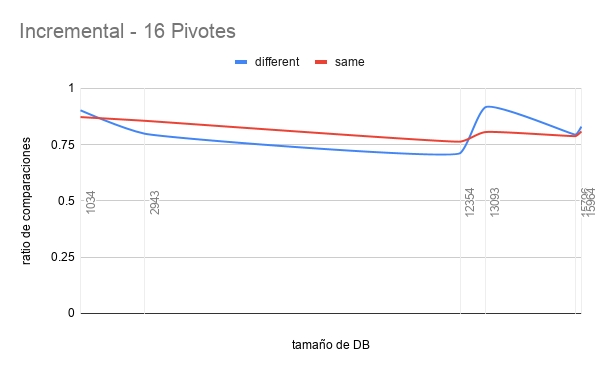
\includegraphics[width=0.8\textwidth]{imagenes/same-vs-diff-Incremental-16Pivotes.png}
		\caption{\small Estrategia de selecci\'on incremental para 16 pivotes: mismos pivotes vs diferentes}
		\label{fig:same-vs-diff-Incremental-16Pivotes}

		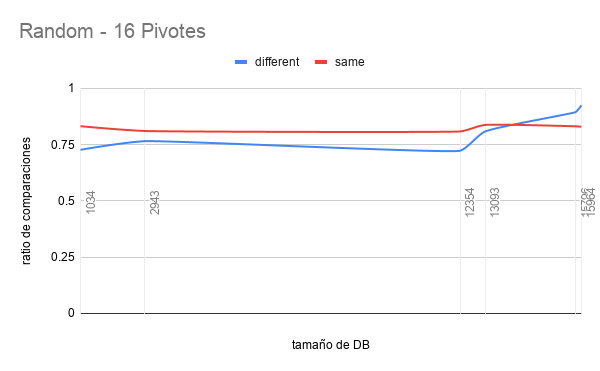
\includegraphics[width=1\textwidth]{imagenes/same-vs-diff-Random-16Pivotes.png}
		\caption{\small Estrategia de selecci\'on random para 16 pivotes: mismos pivotes vs diferentes}
		\label{fig:same-vs-diff-random-16Pivotes}	
	\end{center}
\end{figure}

\begin{figure}[H]
	\begin{center}
		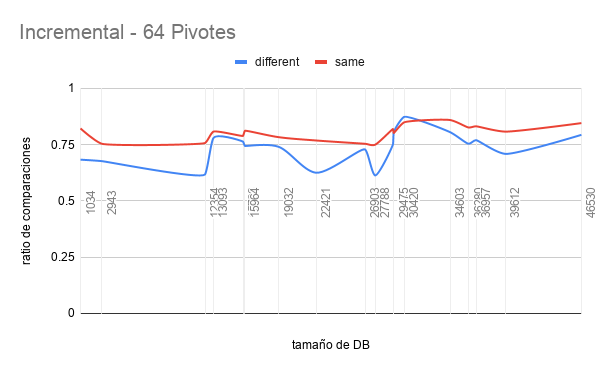
\includegraphics[width=1\textwidth]{imagenes/same-vs-diff-Incremental-64Pivotes.png}
		\caption{\small Estrategia de selecci\'on incremental para 64 pivotes: mismos pivotes vs diferentes}
		\label{fig:same-vs-diff-Incremental-64Pivotes}
		
		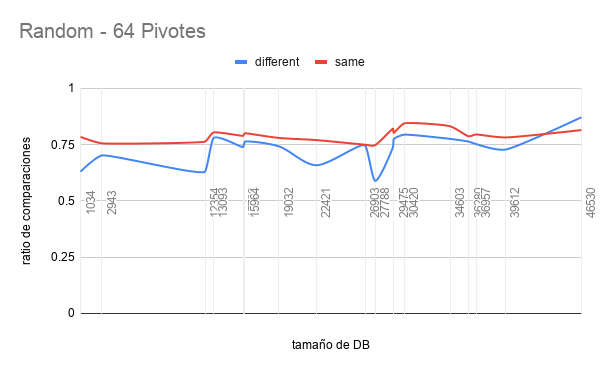
\includegraphics[width=1\textwidth]{imagenes/same-vs-diff-Random-64Pivotes.png}
		\caption{\small Estrategia de selecci\'on random para 64 pivotes: mismos pivotes vs diferentes}
		\label{fig:same-vs-diff-random-64Pivotes}
	\end{center}
\end{figure}

Por lo que se puede observar, aunque la estrategia var\'ia por cada base de datos, en t\'erminos generales se comporta mejor la pol\'itica de selecci\'on  \textit{diferentes grupos pivotes por categor\'ia o base de datos} para ambas t\'ecnicas; random e incremental.\\


\section{Ejecuci\'on experimental}

En una segunda etapa,  nos concentramos en c\'omo agrupar los datos teniendo en cuenta la variaci\'on del tama\~no de las bases de datos para luego poder analizar la informaci\'on segmentada y poder sacar mejores conclusiones.\\

\subsection{Creaci\'on de grupos}

Dada la variabilidad de tamaños de las bases de datos, para poder analizar luego los resultados correctamente, definimos cuatro grupos segmentados por el tamaño de base de datos y por cantidad de pivotes. Esto es, calculamos el ratio de pivotes sobre el tamaño de las base de datos (DB), quedando la siguiente distribuci\'on:\\

\begin{table}[htbp]
\begin{center}
\begin{tabular}{|p{1.1cm}|p{1.8cm}|p{3.2cm}|p{2.2cm}|p{2.5cm}|}
\hline
Grupo & 
Cantidad de DB & 
Rango del tama\~no de DB & 
N\'umero de Pivotes &  
Cantidad de Experimentos\\
\hline \hline
1 & 
6 & 
[1.034 - 15.964] & 
16, 32, 64, 128, 256 & 
60  \\ \hline
2 &
12 &
[19.032 - 46.530] &
64, 128, 256, 512, 1024 &
120  \\ \hline
3 &
8 &
[57.198 - 13.6323] &
256, 512, 1024, 2048 &
64  \\ \hline
4 &
4 &
[16.7995- 21.3578] &
512, 1024, 2048, 4096 &
32  \\ \hline
\end{tabular}
\caption{Tabla de grupos.}
\label{tabla:grupos}
\end{center}
\end{table}

En total se ejecutaron 276 experimentos. Esto es, 138 experimentos usando t\'ecnica de selecci\'on de pivotes random y 138 experimentos usando t\'ecnica de selecci\'on de pivotes incremental.\\

Se seleccion\'o al azar el 10\% de los elementos de cada una de las bases de datos para realizar las b\'usquedas. La cantidad total de b\'usquedas por rango realizadas fue: 339.899. Este valor incluye las b\'usquedas usadas para descartar la pol\'itica de selecci\'on \textit{Mismo grupo de pivotes para todas las categor\'ias o bases de datos} mencionada anteriormente.\\

\section{An\'alisis de resultados}

Vamos a presentar los resultados segmentados en cuatro grupos y analizaremos tres enfoques diferentes.\\

\subsection{Efecto de la cantidad de pivotes}

Llamaremos ratio de comparaciones al porcentaje de comparaciones respecto del tamaño de la base de datos, esto es porcentaje de filtrado.\\

Las figuras 5.3.x.y muestran el efecto de la cantidad de pivotes sobre el ratio de comparaciones por cada base de datos para los distintos grupos. Cada una de las l\'ineas es una base de datos, y estas bases de datos est\'an representadas por su tamaño como se muestra en las gr\'aficas.\\

GRAFICAs

grupo 1

GRAFICA: Efecto de la cantidad de pivotes sobre el ratio de comparaciones. T\'ecnica de selecci\'on de pivotes random


GRAFICA: Efecto de la cantidad de pivotes sobre el ratio de comparaciones. T\'ecnica de selecci\'on de pivotes incremental

grupo2
grupo 3
grupo 4 

END graficas

conclusiones:
Se puede observar que para todas las DB de los diferentes grupos a medida que aumenta el n\'umero de pivotes, el porcentaje de comparaciones es menor.\\

\subsection{Efecto tamaño de la base de datos}

En las figuras 5.4.x.y mostraremos el efecto del tamaño de la base de datos sobre el ratio de comparaciones por pivotes. Tambi\'en mostraremos los resultados segmentado seg\'un los grupos antes mencionados.\\

GRAFICAS

grupo 1

GRAFICA: Efecto del tamaño de la base de datos sobre el ratio de comparaciones por pivotes. T\'ecnica de selecci\'on de pivotes random

GRAFICA:  Efecto del tamaño de la base de datos sobre el ratio de comparaciones por pivotes. T\'ecnica de selecci\'on de pivotes incremental


grupo2
grupo 3
grupo 4 

END graficas

conclusiones:
Se observa que a medida que aumenta el tamaño de la base de datos, disminuye el porcentaje de filtrado para los distintos grupos de pivotes, en otras palabras aumenta el porcentaje de comparaciones respecto del tamaño de la base de datos.\\

\subsection{Efecto de las t\'ecnicas de selecci\'on de pivotes}

En las figuras 5.5.x.y comparamos las t\'ecnicas de selecci\'on de pivotes, random e incremental, usando como m\'etrica el n\'umero de evaluaciones de distancia para cada unos de los pivotes. De cada grupo mostraremos a continuaci\'on solo las base de datos de mayor tamaño; el resto se adjuntan en el anexo XX.\\

GRAFICAS POR GRUPOS

 GRAFICA: Efecto de las t\'ecnicas de selecci\'on de pivotes random vs incremental respecto de evaluaciones de distancia
 
 conclusiones:
 Como se puede observar, solo en el grupo 1; la t\'ecnica de selecci\'on incremental realiza menos cantidad de evaluaciones de distancia. En los grupos 2, 3 y 4 es mejor la t\'ecnica de selecci\'on random solo por muy poca diferencia.\\
 
 
Dado que el comportamiento para ambas t\'ecnicas de selecci\'on no era el que esperabamos, es decir, incremental no era mucho mejor que random en cuanto a ratio de comparaciones, hicimos un an\'alisis emp\'irico sobre diferentes categor\'ias para entender tal comportamiento. 




 